\documentclass[aspectratio=169,10pt]{beamer}
\usepackage[utf8]{inputenc}
\usepackage[T1]{fontenc}
\usepackage{amsmath,amssymb}
\usepackage{graphicx}
\usepackage{booktabs}

\definecolor{Ink}{HTML}{172B3A}
\definecolor{Navy}{HTML}{183B56}
\definecolor{Teal}{HTML}{087E8B}
\definecolor{Gold}{HTML}{D99A2B}
\definecolor{Mist}{HTML}{EEF4F6}
\definecolor{Alert}{HTML}{B23A48}

\usetheme{default}
\setbeamertemplate{navigation symbols}{}
\setbeamertemplate{itemize item}{\color{Teal}$\blacktriangleright$}
\setbeamertemplate{itemize subitem}{\color{Gold}$\bullet$}
\setbeamercolor{normal text}{fg=Ink,bg=white}
\setbeamercolor{frametitle}{fg=white,bg=Navy}
\setbeamercolor{structure}{fg=Teal}
\setbeamerfont{frametitle}{series=\bfseries,size=\large}
\setbeamersize{text margin left=0.55cm,text margin right=0.55cm}
\setbeamertemplate{footline}{%
  \leavevmode\hbox{%
  \begin{beamercolorbox}[wd=.82\paperwidth,ht=2.6ex,dp=1.1ex,leftskip=.55cm]{author in head/foot}%
    \color{Navy}\scriptsize Acemoglu, Kong \& Ozdaglar (2026) \enspace\textcolor{Teal}{|}\enspace Repository 4
  \end{beamercolorbox}%
  \begin{beamercolorbox}[wd=.18\paperwidth,ht=2.6ex,dp=1.1ex,rightskip=.55cm plus1fil]{date in head/foot}%
    \color{Navy}\scriptsize\hfill\insertframenumber/\inserttotalframenumber
  \end{beamercolorbox}}}

\newcommand{\paperlabel}{\textcolor{Navy}{\scriptsize\bfseries PAPER RESULT}}
\newcommand{\extlabel}{\textcolor{Alert}{\scriptsize\bfseries OUR PROPOSED EXTENSION --- NOT IN THE PAPER}}
\newcommand{\softbox}[1]{\begin{beamercolorbox}[rounded=true,sep=.6em]{block body}#1\end{beamercolorbox}}
\setbeamercolor{block body}{fg=Ink,bg=Mist}

\title{AI, Human Cognition and Knowledge Collapse}
\subtitle{Acemoglu, Kong \& Ozdaglar (2026)}
\author{}
\date{}

\begin{document}

\begin{frame}[plain]
  \vspace{.7cm}
  {\color{Teal}\rule{1.8cm}{3pt}}\par
  \vspace{.45cm}
  {\color{Navy}\fontsize{25}{29}\selectfont\bfseries
    AI, Human Cognition and\\ Knowledge Collapse\par}
  \vspace{.35cm}
  {\large Acemoglu, Kong \& Ozdaglar (2026)}\par
  \vspace{.75cm}
  {\color{Ink}NBER Working Paper 34910 \enspace\textcolor{Teal}{|}\enspace February 2026}\par
  \vfill
  \href{https://github.com/carlosgomezp28/ai-04-acemoglu}{%
    \color{Teal}\texttt{github.com/carlosgomezp28/ai-04-acemoglu}}
  \vspace{.35cm}
\end{frame}

\begin{frame}{Paper and the agent's problem}
  \paperlabel
  \vspace{.12cm}

  \softbox{\small Human learning creates private context-specific information and general
  knowledge for future cohorts; agentic AI directly supplies context-specific precision.}

  \vspace{.25cm}
  \begin{columns}[T,onlytextwidth]
    \begin{column}{.39\textwidth}
      \textbf{Information and production}
      \[
        Y=\sigma^{-2}+\lambda_I e+\tau_A.
      \]
      \begin{beamercolorbox}[rounded=true,sep=.55em]{alerted text}
        \centering Assumption 1
        \[
          \Delta_I=0,\qquad \Delta_X>0.
        \]
      \end{beamercolorbox}
      \vspace{.12cm}
      \scriptsize
      \[
        \Delta_I=f(0,1)-f(0,0).
      \]
      Thus context-specific knowledge alone has no incremental productive value.
    \end{column}

    \begin{column}{.58\textwidth}
      \textbf{Static choice of human effort}
      \[
      \max_{e\ge 0}\left\{
      f(0,0)+\Delta_GG(X)+\Delta_XG(X)G(Y)
      -\frac{e^\alpha}{\alpha}\right\}.
      \]
      \vspace{-.2cm}
      \[
        \boxed{\Delta_XG(X)\lambda_I g(Y)=e^{\alpha-1}}
      \]
      \vspace{-.05cm}
      \begin{beamercolorbox}[rounded=true,sep=.5em]{block body}
      \scriptsize
      \begin{tabular}{@{}ll@{}}
        $X$ & general-knowledge precision \\
        $e$ & human learning effort \\
        $\tau_A$ & agentic-AI precision \\
        $Y$ & total context-specific precision
      \end{tabular}
      \end{beamercolorbox}
    \end{column}
  \end{columns}
\end{frame}

\begin{frame}{Observation 1: complements and substitutes}
  \paperlabel
  \vspace{.15cm}

  \begin{columns}[T,onlytextwidth]
    \begin{column}{.49\textwidth}
      \begin{beamercolorbox}[rounded=true,sep=.65em]{block body}
        \centering\textbf{General knowledge complements effort}
        \[
          \boxed{U_{eX}=\Delta_X\lambda_I g(X)g(Y)>0}
        \]
        \scriptsize\textbf{Strict when}\par
        $\Delta_X>0,\ \lambda_I>0,\ X>0,\ Y>0,$\\
        $g(X)>0,\ g(Y)>0.$

        \vspace{.12cm}
        \footnotesize $X\uparrow\Rightarrow$ marginal return to effort $\uparrow$.
      \end{beamercolorbox}
    \end{column}
    \begin{column}{.49\textwidth}
      \begin{beamercolorbox}[rounded=true,sep=.65em]{block body}
        \centering\textbf{Agentic AI substitutes for effort}
        \[
          \boxed{U_{e\tau_A}=\Delta_XG(X)\lambda_Ig'(Y)<0}
        \]
        \scriptsize\textbf{Strict when}\par
        $\Delta_X>0,\ \lambda_I>0,\ X>0,\ Y>0,$\\
        $G(X)>0,\ g'(Y)<0.$

        \vspace{.12cm}
        \footnotesize $\tau_A\uparrow\Rightarrow$ marginal return to effort $\downarrow$.
      \end{beamercolorbox}
    \end{column}
  \end{columns}

  \vspace{.25cm}
  \begin{beamercolorbox}[rounded=true,sep=.6em]{alerted text}
    \small\textbf{Welfare trap.} Holding $X$ fixed, more accurate AI raises
    static payoff; by crowding out learning and future general knowledge, it need
    not raise long-run welfare monotonically.
  \end{beamercolorbox}
\end{frame}

\begin{frame}{What I did}
  \begin{columns}[T,onlytextwidth]
    \begin{column}{.41\textwidth}
      \paperlabel
      \vspace{.12cm}
      \begin{beamercolorbox}[rounded=true,sep=.6em]{block body}
      \textbf{Paper reproduction}
      \begin{itemize}\footnotesize
        \item reconstructed the static objective and FOC;
        \item derived Observation 1 and checked boundaries;
        \item audited all three Section 5 extensions;
        \item isolated the maintained production restriction
          \[\Delta_I=0;\]
        \item compiled algebraic sign checks in \texttt{lean/Main.lean}.
      \end{itemize}
      \end{beamercolorbox}
    \end{column}

    \begin{column}{.57\textwidth}
      \extlabel
      \vspace{.12cm}
      \begin{beamercolorbox}[rounded=true,sep=.55em]{block body}
      \small
      \[
      \Delta_I>0,\quad \Delta_X>0,\quad
      \Delta_G=1-\Delta_I-\Delta_X\ge0.
      \]
      \[
        \boxed{[\Delta_I+\Delta_XG(X)]\lambda_Ig(Y)=e^{\alpha-1}}
      \]
      \footnotesize\textbf{Boundary.} The paper has $X=0\Rightarrow e^*=0$.
      In our extension,
      \[
        \Delta_I>0,\ \lambda_I>0,\ \alpha>1,\quad
        \sigma^{-2},\tau_A<\infty
        \quad\Rightarrow\quad e^*(0,\tau_A)>0.
      \]
      \textbf{Public knowledge.} Given this positive boundary effort,
      \[
        \lambda_G>0,\ I>0,\ 0\le\Sigma^2<\infty
        \quad\Rightarrow\quad F_{\Delta_I}(0)>0.
      \]
      \end{beamercolorbox}
    \end{column}
  \end{columns}

  \vspace{.2cm}
  \begin{beamercolorbox}[rounded=true,sep=.55em]{block body}
    \centering\bfseries Exact zero public knowledge is no longer a fixed point
    for finite AI precision.
  \end{beamercolorbox}
\end{frame}

\begin{frame}{Where I did not believe AI}
  \begin{columns}[T,onlytextwidth]
    \begin{column}{.56\textwidth}
      \centering
      \includegraphics[page=3,width=.96\linewidth,trim=22 355 22 18,clip]{hand/extension-derivation.pdf}
      \par
      {\tiny Handwritten audit: \texttt{hand/extension-derivation.pdf}, p.~3}
    \end{column}

    \begin{column}{.42\textwidth}
      \extlabel
      \vspace{.08cm}
      \begin{beamercolorbox}[rounded=true,sep=.5em]{alerted text}
        \centering\scriptsize\textbf{INITIAL AI CLAIM}
        \[
          \Delta_I>0\Rightarrow\text{knowledge collapse is eliminated.}
        \]
        {\color{Alert}\bfseries TOO STRONG.}
      \end{beamercolorbox}

      \vspace{.08cm}
      \begin{beamercolorbox}[rounded=true,sep=.5em]{block body}
        \centering\scriptsize\textbf{AUDITED VERDICT}
        \[
          \boxed{\Delta_I>0\Rightarrow F_{\Delta_I}(0)>0}
        \]
      \end{beamercolorbox}

      \vspace{.1cm}
      \footnotesize Exact zero disappears, but low positive states, multiplicity,
      path dependence, and welfare loss may remain.

      \vspace{.1cm}
      \scriptsize\textbf{Section 5.2:} synthetic data adds exogenous public
      precision; ours works through endogenous human effort.
    \end{column}
  \end{columns}
\end{frame}

\end{document}
